\documentclass{article}

\usepackage{ragged2e}
\usepackage{graphicx}
\usepackage{amsmath}
\usepackage{siunitx}
\usepackage{hyperref}

\renewcommand{\c}[1]{\texttt{#1}}

\begin{document}

%\begin{flushright}
    \noindent
    Rodrigo Becerril Ferreyra\\
    CECS 361 Section 01\\
    Lab 1\\
    Date: 10 September 2020
%\end{flushright}

\section{Introduction} The purpose of this lab is to get
familiar with the Vivado workflow and to demonstrate knowledge
of topics that were covered in class. Specifically, we were
instructed to create a four-bit array multiplier
in Verilog. An array
multiplier is a circuit that takes two inputs---in this case,
two four-bit numbers---and multiplies them to get the
product. This is achieved by using the standard long multiplication
algorithm (details can be found at
\url{https://en.wikipedia.org/wiki/Multiplication_algorithm#Long_multiplication}).
In the case of the binary number system, this algorithm can be
simplified by the fact that the multiplication table is very
simple:

\begin{figure}[h]
    \centering
    \begin{tabular}{c | c c}
        X    & \num{0} & \num{1} \\ \hline
        \num{0} & \num{0} & \num{0} \\
        \num{1} & \num{0} & \num{1}
    \end{tabular}
    \caption{Base-2 multiplication table.}
\end{figure}

Specifically, if the multiplicand (henceforth \c{B}) is \num{1}, then
the multiplier (henceforth \c{A}) can be copied down as a partial product; if
\c{B} is \num{0}, then zeros can be
copied down instead. This fact is exploited in the making of a
hardware-based array multiplication circuit.

\section{Implementation} The implementation of this
multiplier circuit relies on two parts: the generation
of partial products, and the addition of those partial
products. Part 1 can be achieved using multiplexers,
and Part 2 can be achieved using half-adders and
full-adders.

\subsection{Partial Products} As previously stated,
the partial products can be generated by using a multiplexer.
The LSB of \c{B} is fed into the
selection input of the
first array of multiplexers. If
\c{B[0]} is \num{0}, then a \num{0} is placed into the
partial product; if \c{B[0]} is \num{1}, then \c{A} is
placed into the partial product instead.
For the next partial product, \c{B[1]} was fed into the next set of four
multiplexers' select input, and so on.
This is done
simultaneously for all
four rows of multiplexers,
which takes \num{16}
\(2\text{-to-}1\) one-bit multiplexers in total.

\subsection{Adding the Partial Products} Given only one-bit
half-adders and full-adders to work with, adding up all of
the partial products is a messy task which involves lots of
wires and adders. It is possible to derive the exact circuit
which allows the addition of all partial products while taking
into account the long multiplication algorithm, which calls
for the shifting of the place value of the LSB one to the right
for every partial product. However, we were given this circuit
so there was no need to.

\section{Testing and Verification} Once the main module was
completed, the time for testing arrived. I created a nested loop
that would loop through all \num{256} possible values
for \num{2} four-bit numbers \c{A} and \c{B}. In each iteration,
I defined a wire named \c{expected\_product}, which
was set to \c{A*B}. If the product that came from the
unit under test did not match this expected product, then
an error message would print. However, the simulation
ran smoothly and no error was printed. Below is a screenshot
of a portion of the timing diagram that was produced; note
that the values are represented in unsigned decimal.

\begin{figure}[h]
    \centering
    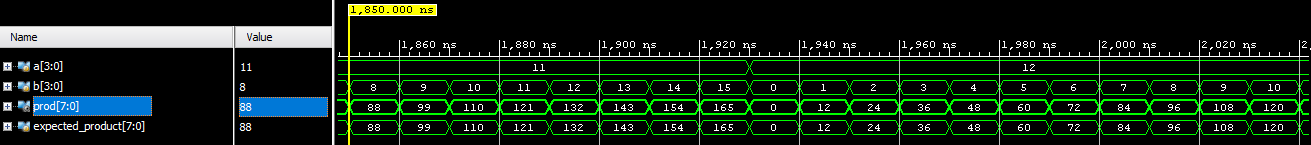
\includegraphics[width=\textwidth]{Images/waveform.png}
    \caption{Small snippet of waveform comparing the calculated product \c{prod} with the expected product.}
\end{figure}

Here is a small table of several test values. Note that the
values are represented in binary.

\begin{figure}[h]
    \centering
    \begin{tabular}{c | c | c}
        Multiplier (\c{A}) & Multiplicand (\c{B}) & Product (\c{prod}) \\ \hline
        \c{1101} & \c{1001} & \c{0111\_0101} \\
        \c{0010} & \c{1111} & \c{0001\_1110} \\
        \c{1101} & \c{1011} & \c{1000\_1111} \\
        \c{1111} & \c{0110} & \c{0101\_1010} \\
        \c{0011} & \c{1010} & \c{0001\_1110}
    \end{tabular}
    \caption{Table of values.}
\end{figure}

\end{document}
